\section{Struttura dei Dischi}
Da una parte è possibile suddividere un singolo disco in più dischi virtuali, detti \textbf{partizioni} o \textbf{minidischi}.

Una partizione che contiene un file system è detta \textbf{volume} e possiede una directory di dispositivo che contiene informazioni di tutti i file della partizione.

\begin{figure}[H]
    \centering
    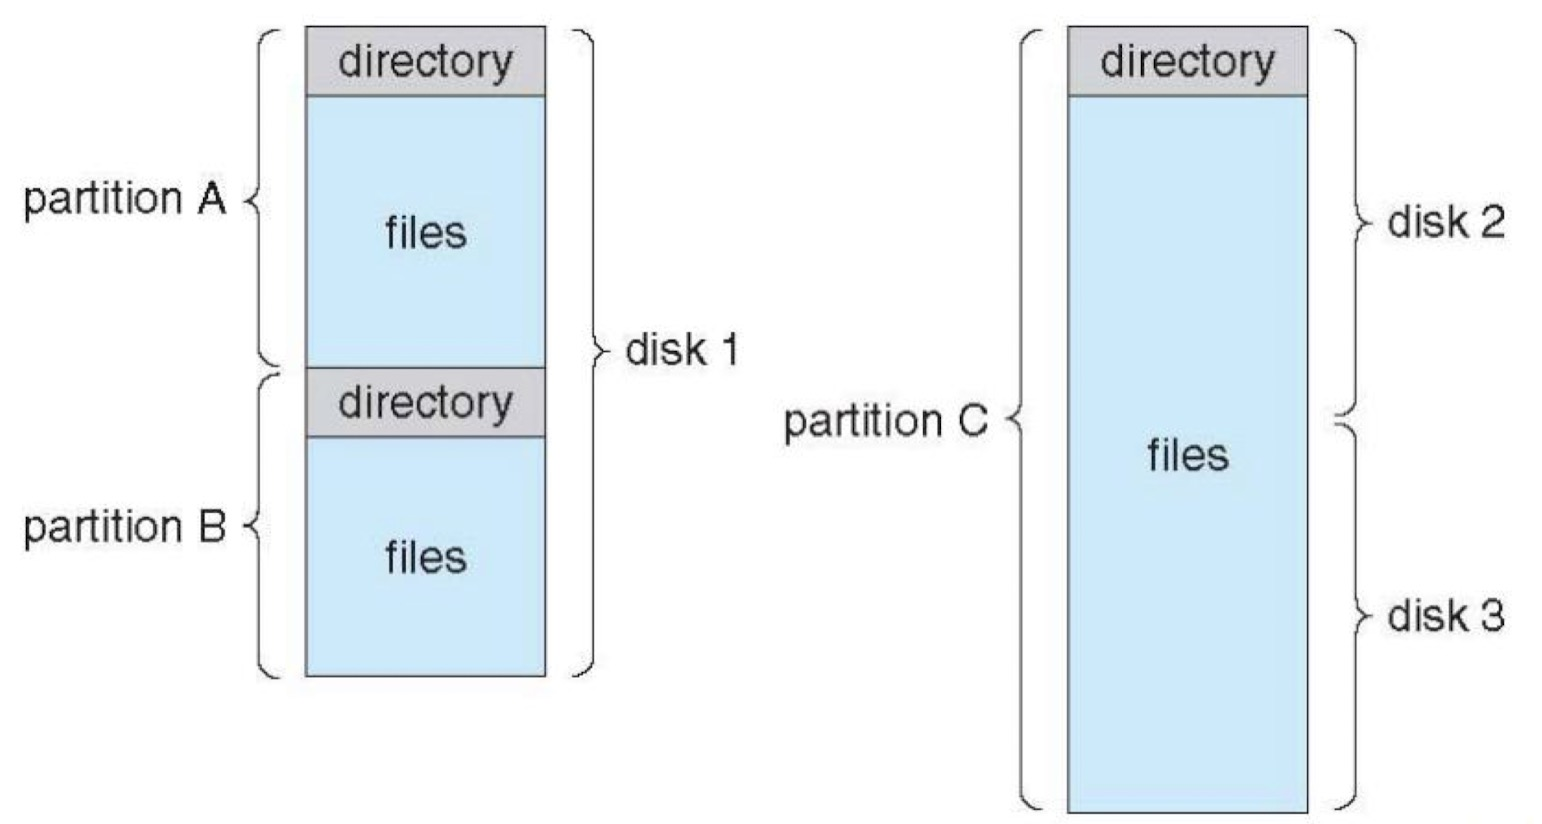
\includegraphics[width=0.5\linewidth]{assets/partizioni.jpg}
\end{figure}

\spacer
Dall'altra è possibile unire più dischi per creare un disco virtuale con specifiche proprietà mediante RAID che vedremo alla fine del capitolo.

\subsection{Formattazione}
Oltre alla formattazione logica, ovvero la creazione di un file system sul disco, esiste la \textbf{formattazione fisica} o di basso livello.

La formattazione prevede il salvataggio di una struttura dati che associa ogni settore fisisco ad un settore logico, permettendo così anche la gestione degli errori, quando un settore è difettoso esso viene rimosso dalla struttura dati, rendendo ancora possibile l'utilizzo del disco.

\subsection{Correzione degli errori}
Le memorie fisiche utilizzano tecniche di memorizzazione che possono generare errori.
Definiamo $C$ come la codifica corretta e $C'$ la codifica effettiva, la \textbf{distanza di Hamming} $H(C, C')$ è il numero di bit sbagliati nella codifica effettiva.

\spacer
Per rilevare questi errori è necessario aggiungere dei bit di parità alla codifica. In particolare vogliamo aggiungerne un numero tale da permetterci di rilevare non solo se ci sono errori, ma anche quali bit sono errati. In questo modo è possibile non solo rilevare gli errori, ma anche correggerli.

Per fare ciò utilizziamo dei bit di parità che coprano ognuno un diverso gruppo di bit, così da poter individuare il dato errato.
Per sapere su quali bit di parità influisce il bit k basta riscriverlo come somma di potenze di 2, quindi $7 = 1 + 2 + 4$

\begin{figure}[H]
    \centering
    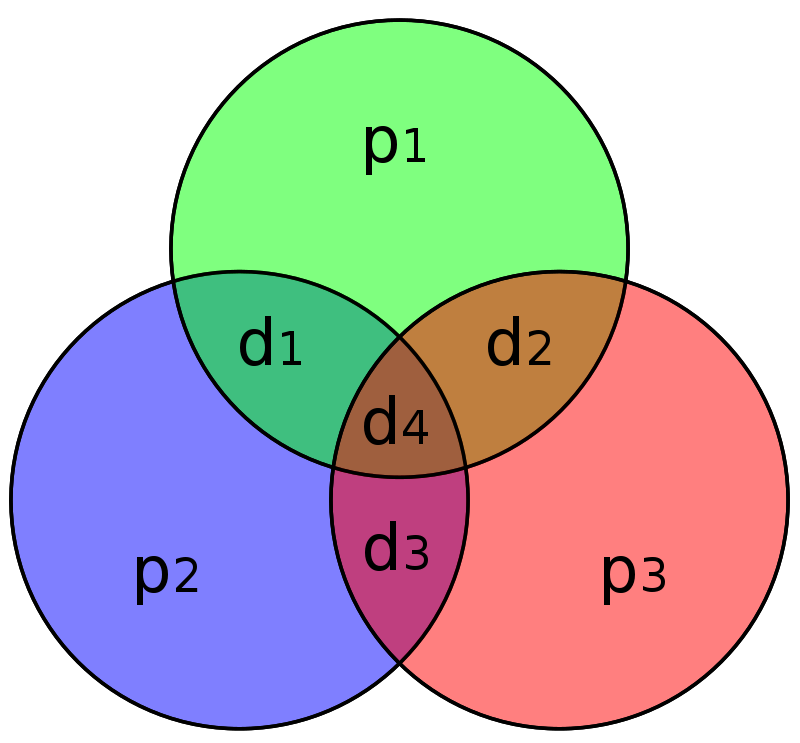
\includegraphics[width=0.35\linewidth]{assets/hamming-diagram.png}
\end{figure}

In questo caso se, ad esempio, i bit $p_1$ e $p_3$ ci segnalano un errore sappiamo che sicuramente il dato $d_2$ è errato.

\spacer
Per rilevare $d$ errori è necessario utilizzare $d+1$ bit, mentre per correggere lo stesso numero di errori vanno utilizzati $2d+1$ bit.

I bit di parità vengono poi confrontati tra la sequenza iniziale e quella effettivamente scritta, se ci sono discrepanze sappiamo che ci sono degli errori e, in caso, possiamo trovare i bit colpevoli.


\subsubsection*{Esempio}
Se vogliamo rilevare gli errori sulla sequenza: \texttt{0 1 1 0}

\spacer
Inseriamo dei bit di parità in posizione 1, 2, 4: \texttt{- - 0 - 1 1 0}

Il bit 3 influenza 1 e 2 (3 = 1+2), (5 = 1+4), (6 = 2+4), (7 = 1+2+4)

\spacer
Per calcolare i bit di parità: 1 se il numero di 1 è dispari, 0 se pari.

Quindi, ad esempio, il bit 1 è influenzato dai bit 3, 5, 7 ($\texttt{0 1 0} \Rightarrow 1$)

Otteniamo: \texttt{1 1 0 0 1 1 0}
